\section{Auditor Extension} \label{sec:auditor}
Until now we have not \emph{verified} whether the certificate chain of an SFO is
publicly logged as promised by the issued SCTs.  As such, it is unlikely that a
misbehaving CT log will be detected.
Our base design can be extended to follow-up
on an SFO's inclusion status rather than adding the underlying certificate chain
to another CT log.  This has the benefit of relaxing our initial trust
assumption, namely that some CT logs are honest, as well as making it possible
to disclose those CT logs that are dishonest.  The downside is added
complexity, which introduces additional threats that must be considered.

\subsection{Design Sketch} \label{sec:auditor:design}
Figure~\ref{fig:auditor} provides an overview of the extended design.  Tor
Browser submits presented SFOs probabilistically to CTRs that are selected at
random, and CTRs store the submitted SFOs before any auditing takes place.
Here, auditing refers to inclusion verification rather than adding certificate
chains.  The moment before auditing, the SFO in question is shared with a CTR
that acts as a \emph{watchdog}.  Unless the auditing CTR receives a timely
inclusion proof and acknowledges it to its watchdog, the (now suspicious) SFO is
reported to a CT auditor.  Phase~1 remains unchanged, some changes are needed
in phase~2, and major changes are required in phase~3 as well as the Tor
consensus.  The extra-info document also includes two new metrics that are
related to flooding.

\begin{figure*}
    \centering
	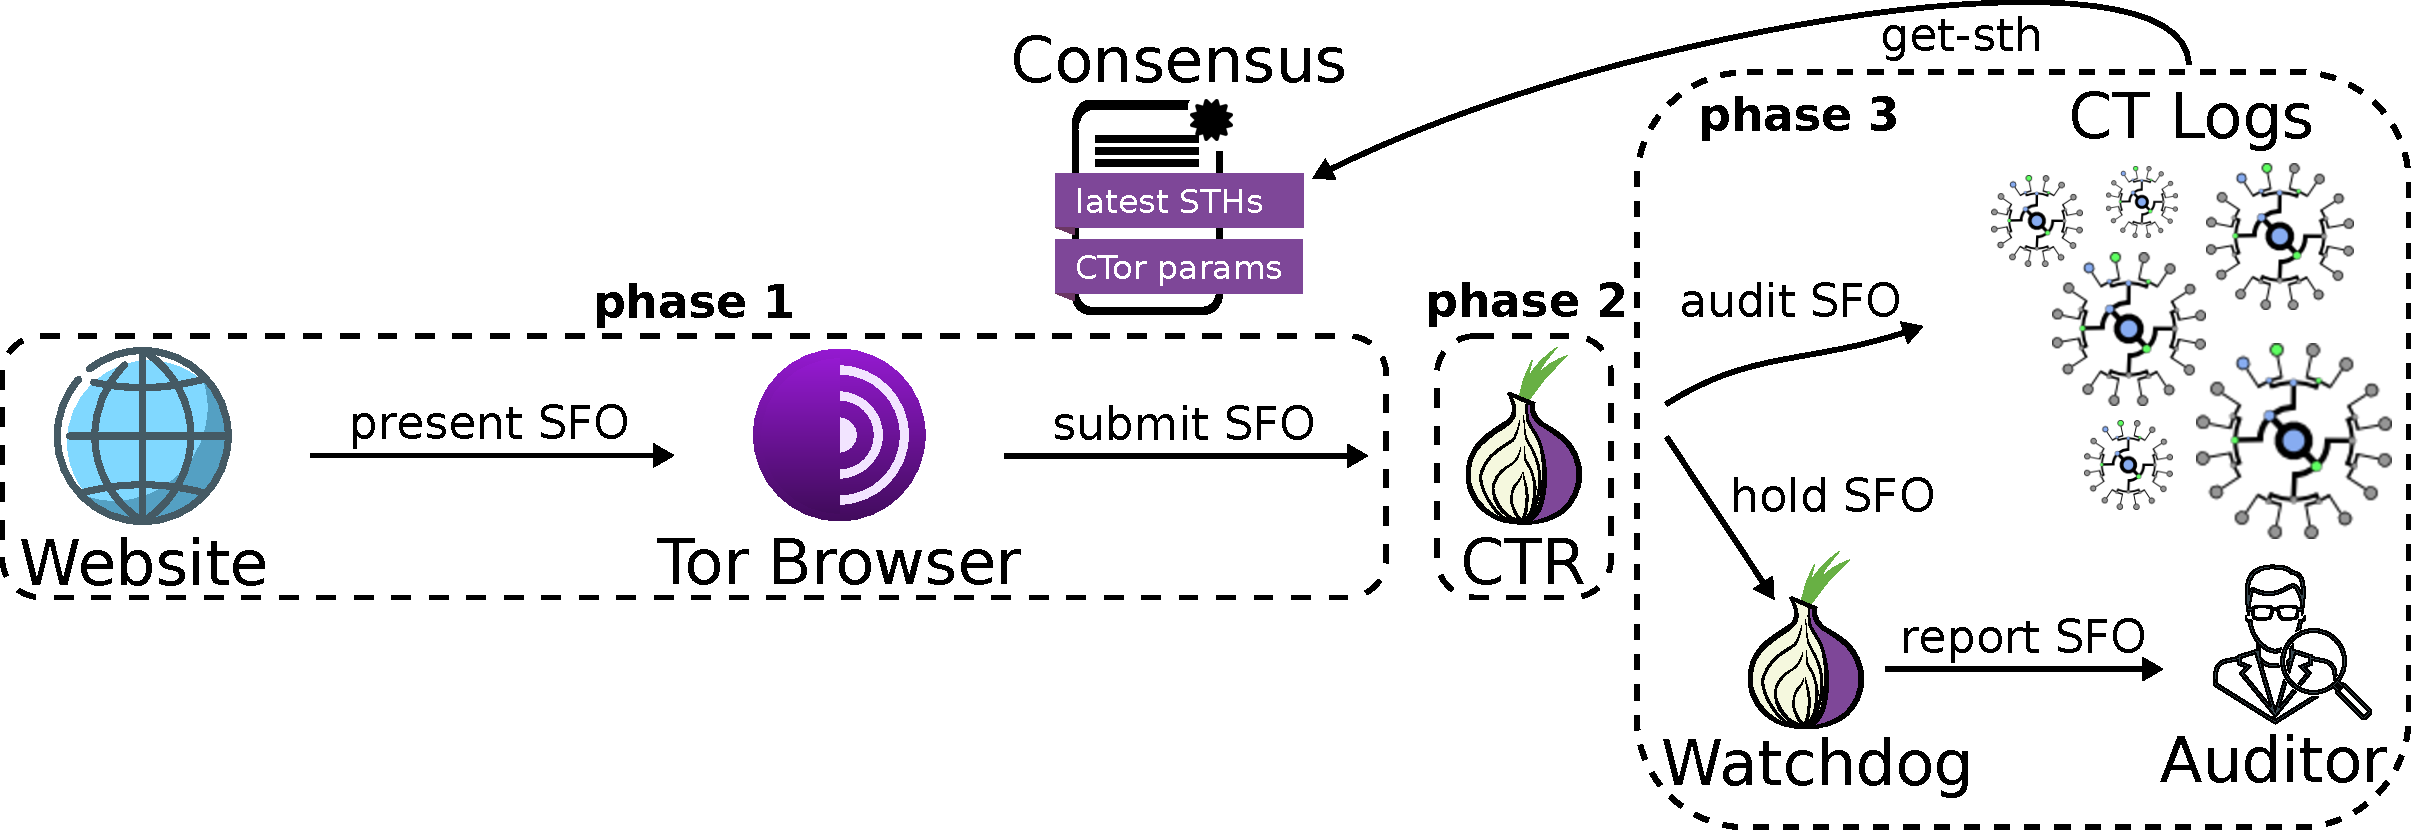
\includegraphics[width=0.8\textwidth]{img/design-auditor}
	\vspace{-8px}
	\caption{The auditor extension, where cryptographic evidence of log omission
	can be collected. The extension changes the consensus to include the latest
	STHs from CT logs. The CTRs in phase 3 now challenge logs to prove inclusion
	of certificates from SFOs, using other CTRs as ``watchdogs'', ensuring that
	SFOs that are not provably correct are reported to trusted auditors.}
	\label{fig:auditor}
	\vspace{-10px}
\end{figure*}

\subsubsection{Tor Consensus} \label{sec:auditor:design:consensus}
Tor's consensus should capture a fixed view of the CT landscape by publishing
STHs from all recognized logs.  A CT log is recognized if a majority of directory
authorities proposed a \texttt{ct-log-info} item, which contains a log's ID,
public key, base URL, MMD, and most recent STH.  Each directory authority
proposes its own STH, and agrees to use the most recent STH as determined by
timestamp and lexicographical order.  Since CTRs verify inclusion with regards
to SCTs that TB accepts, the CT logs recognized by TB must be
in Tor's consensus.

Tor's directory authorities also majority-vote on \texttt{ct-auditor} items,
which pin base URLs and public keys of CT auditors that watchdogs contact in
case that any log misbehavior is suspected.  A watchdog triggers if the time
specified by \texttt{ct-watchdog-timeout} elapses without receiving any
acknowledgment.  The following auditor submission is governed by a
\texttt{ct-auditor-timeout}, which, if triggered, results in a resubmission
later on.

\subsubsection{Phase~2---Storage} \label{sec:auditor:design:phase2}
Other than updating the criteria of what it means that an SFO can be audited
in phase~3, the computation of $l$ and $t$ changes for a buffer's entry.  With
regards to some CT circuit, process an incoming SFO $s$ as follows:
\begin{enumerate}
	\item\label{enm:ext:storage:close} Close the current circuit to enforce
		one-time usage.
	\item\label{enm:ext:storage:unrecognized} Discard unrecognized SCTs in $s$
		whose logs have no corresponding \texttt{ct-log-info} items listed in
		the Tor consensus.  Stop if there are no remaining SCTs in~$s$.
	\item\label{enm:ext:storage:cached}
		Stop if $s$ is cached or pending to be audited already.
	\item\label{enm:ext:storage:fix-log} Sample a CT log $l$ that issued a
		remaining SCT in~$s$.
	\item\label{enm:storage:audit-after} Compute an \texttt{audit\_after}
		time~$t$, see Figure~\ref{fig:audit-after}.
	\item\label{enm:storage:store} Add $(l,t,s)$ to a buffer of pending SFOs.
\end{enumerate}

Recall from Section~\ref{sec:background:ct} that an inclusion proof is fetched
with regards to an STH.  As such, we discard SCTs that cannot be verified due to
lack of \texttt{ct-log-info} items in the Tor consensus.  The sampled CT log $l$
now refers to an entity that issued an SCT in the submitted SFO, and it will be
challenged to prove inclusion in phase~3 sometime after the
\texttt{audit\_after} timestamp $t$ elapsed.  Figure~\ref{fig:audit-after} shows
that $t$ takes the log's MMD into account.  This is one of two parts that
prevent \emph{early signals} to the issuing CT logs that an SFO is being
audited.  For example, if an SFO is audited before the MMD elapsed, the issuing
CT log could simply merge the underlying certificate chain to avoid an MMD
violation.  This would not yield any improvement with regards to the base
design.

\begin{figure}
	\centering
	\pseudocode[linenumbering, syntaxhighlight=auto]{%
		\textrm{t} \gets \mathsf{now}() +
			\mathsf{MMD} +
			\mathsf{random}(\texttt{ct-delay-dist}) \\
		\pcif \textrm{SCT.timestamp} + \textrm{MMD} <
				\mathsf{now}():\\
			\pcind\textrm{t} \gets \mathsf{now}() +
				\mathsf{random}(\texttt{ct-delay-dist})
	}
	\caption{%
		Algorithm that computes an \texttt{audit\_after} timestamp $t$.
	}
	\label{fig:audit-after}
\end{figure}

\subsubsection{Phase~3---Auditing} \label{sec:auditor:design:phase3}
In addition to maintaining a single Tor circuit that is used to interact with
CT logs that have \texttt{ct-log-items}, a distinct Tor circuit is maintained
and rotated that ends at a random watchdog CTR.  Given a known CT log
$l$:
\begin{enumerate}
	\item\label{enm:ext:auditing:backoff} Sample a delay $d \gets
	\mathsf{random}(\texttt{ct-backoff-dist})$ and wait until $d$ time units
	elapsed.
	\item Connect to a random watchdog CTR.
	\item\label{enm:auditing:loop} For each pending buffer entry $(l',s,t)$,
	where $l' = l$, $t <= \mathsf{now}()$ and $t <=
	\textrm{STH}.\mathsf{timestamp}$:
		\begin{enumerate}
			\item\label{enm:ext:auditing:watchdog} Share $s$ with the current
				watchdog.
			\item\label{enm:ext:auditing:challenge} Use \texttt{ct-log-timeout}
				and $\textrm{STH}.\mathsf{treesize}$ to set a timer and
				challenge the log to prove inclusion.
				\begin{itemize}
					\item\label{enm:ext:auditing:challenge:success} On valid
						proof: send an acknowledgment to the watchdog, then
						cache $s$ and discard it.
					\item\label{enm:ext:auditing:challenge:fail} On any other
						outcome: discard $s$, close circuit to the watchdog CTR,
						and go to step 1.
				\end{itemize}
		\end{enumerate}
\end{enumerate}

An SFO is not audited for inclusion until the log's MMD elapsed \emph{and} there
is an STH in the Tor consensus that captures it.  As such, a CT log that intends
to omit a certificate chain despite promising to merge it within its MMD will
not get an early signal that a CTR will audit it.
Before auditing, the SFO in question is shared with a watchdog that takes on
the responsibility of reporting suspicious SFOs to the pinned CT auditors.
An SFO is considered suspicious if it is not acknowledged by the log-challenging
CTR as verified within the time specified by \texttt{ct-watchdog-timeout}.  As
argued in Section~\ref{sec:auditor:analysis:phase3}, it is motivated to use a
watchdog:
	the attacker learns which CTR holds the problematic SFO at the time of
		auditing, and
	during the \texttt{ct-log-timeout} actions could then be taken to ensure
		that the SFO does not reach a CT auditor.
A watchdog that receives a suspicious SFO reports it to a random CT auditor,
and resubmits it later on if the \texttt{ct-auditor-timeout} happens to
trigger.  An important detail is that at most one SFO should await per log in
each watchdog circuit, and in the case of resubmissions these are stored as part
of the overall SFO buffer to follow the delete-at-random strategy.

\subsubsection{Extra-Info Document} \label{sec:auditor:extra-info}
Following from the \texttt{audit\_after} timestamp algorithm in
Figure~\ref{fig:audit-after}, an SFO may be stored for at least an MMD.  This
results in a relatively large time window during which the attacker can attempt
to flood all CTRs in hope that a target SFO is \emph{flushed} from the relevant
CTR buffer due to finite memory constraints (Section~\ref{sec:base:phase2}).
The threat of flooding is discussed in
Section~\ref{sec:auditor:analysis:phase2}.  It can be detected if CTRs publish
	\texttt{ct-receive-bytes} and
	\texttt{ct-delete-bytes}
in the extra-info document.  These metrics indicate how many SFO bytes were
received and deleted throughout different time intervals, which is similar to
other extra-info metrics such as \texttt{read-history}.

\subsection{Discussion} \label{sec:auditor:analysis}
We analyze \emph{differences} with regards to the base design in
Section~\ref{sec:base}.  The catastrophic impact level is possible because SFOs
that cannot be timely validated against Tor's view of the CT landscape are
reported.  While trust in CT logs is eliminated, it is shifted towards trusted
CT auditors that endeavour to follow-up on suspected log misbehavior. The
premise of third-party auditors is fundamental in our setting: manually
interacting with the wider CT ecosystem to expose a misbehaving log exceeds what
could reasonably be expected by a relay operator. Another observation is that
these auditors are subject to different operational requirements than a
browser-included CT log, which is somewhat analogous to the base design that
instead permits additional community logs for the sake of diversity of actors in
the ecosystem. Appendix~\ref{app:auditor} provides further details on what would
be reasonable expectations on auditors.

\subsubsection{Phase~2---Storage} \label{sec:auditor:analysis:phase2}
The main difference with regards to the base design is that an SFO can be
stored much longer.  The attacker can maximize the \texttt{audit\_after}
timestamp by using a newly issued SFO, resulting in a storage phase of \emph{at
least} an MMD.  This time can be extended further by delaying issuance of an
STH that would capture the omission:
	a log must produce an STH every MMD~\cite{ct,ct/bis}.
This means that the maximized storage time is in the order of two MMDs; not
considering that it also takes time for an STH to be propagated into the Tor
consensus.  Most logs use an MMD of 24~hours, resulting in an attack window that
ranges from one to two days.  A risk-averse attacker should prefer to use the
lower bound:
	suddenly not issuing any new STH is visible, attracting attention.

Following from Tor's threat model, the mis-issued SFO must be stored in
volatile memory and not to disk.  Two risks emerge as a result of the increased
storage time:
	the CTR in question might be restarted by the operator,
	and the attacker could flood it by submitting a large volume of SFOs.
A risk-averse attacker cannot rely on the former to avoid detection, but the
latter might flush a target SFO from a CTR's memory \emph{if deleted at random}.
Appendix~\ref{app:flush} shows that the number of SFO submissions~$k$ that the
attacker needs to flush a buffer of $n>1$ entries with some probability~$p<1$ is
given by:
\begin{equation} \label{eq:flush}
	k = \frac{\log(1-p)}{\log(1 - \frac{1}{n})}
\end{equation}

It is recommended that a non-exit relay should have at least 512~MB of memory.
If the available bandwidth exceeds 40~Mbps, it should have at least
1~GB~\cite{relay-config}.  Given that these recommendations are lower bounds,
suppose the average memory available to store SFOs is 1~GiB (a conservative
assumption).  Further, our dataset in Section~\ref{sec:performance} shows that
the average SFO is in the order of 6~KiB.  This means that the buffer capacity
is $n \gets 174763$ SFOs. Plugging it into Equation~\ref{eq:flush} for $p \gets
\frac{9}{10}$, the attacker's flood must involve $k \gets 402406$ submissions.
In other words, 2.3~GiB must be transmitted to flush a single CTR,\footnote{% As
a corner case and implementation detail, it is important that TB and
CTRs \emph{reject} SFOs that are bogus in terms of size: it is a trivial DoS
vector to load data indefinitely. Analysis based on, e.g., 1~MiB SFOs also
requires 2.3~GiB of data to flush.} which takes $7.9$--$39.3$~minutes if its
bandwidth is between 8 and 40~Mbps. Thus, it is impractical to flush all CTRs
within minutes.

Metrics reported by the Tor project show that there are over 4000 relays that
match our CTR criteria set in
Section~\ref{sec:base:consensus:ctr-flag}~\cite{relay-by-flag}.  As such, a
network-wide flush involves the transmission of at least 8.99~TiB.  It might
sound daunting at first, but distributed over a day it only requires 0.91~Gbps.
While we cannot avoid early signals to the logs \emph{and} at the same time
prevent flushing without writing anything to disk, it is detectable based on the
extra-info document.  On the flip-side, \emph{not observing any flushing} adds a
large degree of confidence that there are no significant numbers of mis-issued
SFOs.

\subsubsection{Phase~3---Auditing} \label{sec:auditor:analysis:phase3}
The main difference with regards to the base design is that we query the
attacker for inclusion proofs; not an independent CT log.  As such, there is a
time window to act between the time that the attacker learns some CTR audits a
mis-issued SFO and until the \texttt{ct-log-timeout} elapses.  Suppose that the
attacker could identify the CTR in question at the time of auditing, i.e.,
despite our design (re)using a Tor circuit for all inclusion proofs.  Clearly,
the query timeout must be a few seconds to avoid premature auditor reporting.
This leaves a large enough window to simply DoS the CTR in question.  Our design
makes no attempt to hide the CTR's identity while querying the log.  For
example, the attacker can trivially \emph{tag} each CTR by submitting many
distinct SFOs, and upon seeing them in the audit loop the exact identity is
revealed.  We mitigated this threat using a watchdog, sending the SFO upfront
\emph{before} auditing.  The attacker does not know the watchdog identity based
on the same premises that the attacker does not know which CTR stores an
SFO during the storage phase.  It should be noted that the use of watchdog CTRs
give the attacker a \emph{second shot} at being selected at random.

Another difference is that inclusion proofs are based on STHs that the directory
authorities fetch from attacker-controlled CT logs, agreeing on which ones to
use via deterministic rules.  This means that the attacker controls which STHs
go into the Tor consensus.  Once an STH is announced, it follows from Tor's
threat model that it is fixed because a threshold of directory authorities are
benign.  As such, CTRs have access to the same (in)consistent view of the CT
landscape.  Fortunately, any inconsistent view that makes it into the Tor
consensus is trivially detected:
	the announced STHs are public and auditable by anyone.
Therefore, the attacker should be deterred from creating split-views in Tor.
Other user agents could benefit from Tor's audited view of CT logs.

% MISC notes
% - Network-wide flush, detectable but hard to attribute
% - Requires new reliable auditor software
% - Bit more bandwidth due to watchdog.  The overhead, when compared to log a
% log extension, is sending an SCT hash and receiving a proof (2-3KiB).
% - A rational attacker is the issuer of all SCTs in the omitted SFO, so it is
% sufficient to verify inclusion with regards to one SCT and then leave it to
% the auditors to bust all involved CT logs.
